\documentclass[border=6pt]{standalone}
\usepackage{fontspec}
\usepackage{tikz}
\usetikzlibrary{positioning,calc}
\definecolor{navy}{HTML}{203A93}
\definecolor{Fred}{HTML}{D33B2F}
\definecolor{sblue}{HTML}{DCEAF7}
\definecolor{sred}{HTML}{F9E1DF}
\begin{document}
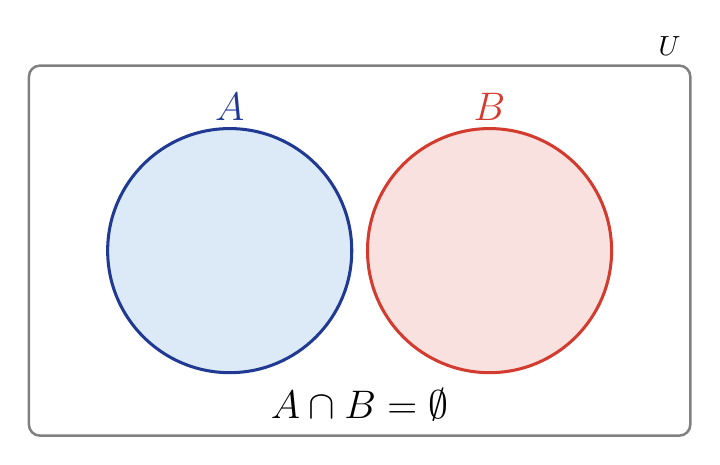
\begin{tikzpicture}[font=\itshape]
  \def\r{1.55}
  \coordinate (A) at (-1.65,0);
  \coordinate (B) at (1.65,0);
  \fill[sblue] (A) circle (\r);
  \fill[sred] (B) circle (\r);
  \draw[gray,line width=0.9pt,rounded corners=4pt] (-4.2,-2.35) rectangle (4.2,2.35);
  \node[above left] at (4.2,2.35) {$U$};
  \draw[navy,line width=1.1pt] (A) circle (\r);
  \draw[Fred,line width=1.1pt] (B) circle (\r);
  \node[navy,font=\Large\bfseries] at ($(A)+(0,1.82)$) {$A$};
  \node[Fred,font=\Large\bfseries] at ($(B)+(0,1.82)$) {$B$};
  \node[font=\Large] at (0,-1.95) {$A\cap B=\emptyset$};
\end{tikzpicture}
\end{document}
